\documentclass[10pt,journal]{IEEEtran}
\IEEEoverridecommandlockouts
\usepackage[spanish,es-tabla]{babel}
\renewcommand{\baselinestretch}{1.5}     %interlineado
\usepackage[utf8]{inputenc} 
\usepackage[square,numbers]{natbib}
\bibliographystyle{abbrvnat}
\usepackage{float}                      % para usar [H]
\usepackage[table,xcdraw]{xcolor}
\usepackage{amsmath,amssymb,amsfonts}
\usepackage{graphicx}
\usepackage{textcomp}
\usepackage{xcolor}

\def\BibTeX{{\rm B\kern-.05em{\sc i\kern-.025em b}\kern-.08em
    T\kern-.1667em\lower.7ex\hbox{E}\kern-.125emX}}

%---------------------------------------------------
\begin{document}

\title{Instrumentos de recolección de datos en Informática o en Ciencias de la Computación\\}
%--------------------------------------------
\author{\IEEEauthorblockN{Ciara Mendez Cruz}
\IEEEauthorblockA{\textit{} \\
\textit{Universidad Nacional de Trujillo} \\ 
\textit{Trujillo, Perú} \\
t022700920@unitru.edu.pe}}
\maketitle
%-------------------------------------------
\begin{abstract}
La investigación en informática estudia múltiples dimensiones de la tecnología informática (software, hardware, etc.) y su uso en el mundo real. Investigar en este gran campo consiste en analizar el problema y plantear soluciones innovadoras: un nuevo algoritmo, una nueva arquitectura, etc. Por ello, es necesario la investigación en este campo y sobretodo elegir correctamente el instrumento que se usa para la recolección de datos.
Uno de los instrumentos de recolección de datos en investigaciones de ciencias de la computación que se utilizó fue una aplicación que se implementó para la segmentación de imágenes basada en conglomerados, denominado Algoritmos Genéticos K-medias (AGKM) que permite analizar imágenes que con otros instrumentos sería casi imposible de realizar, por otro lado, otro instrumento usado fue el muestreo sistemático de grilla sobre la ubicación geográfica de los cultivos de palta hasta recolectar un total de 630 muestras enfermas y sanas y para el reconocimiento de estos datos se utilizaron 4 algoritmos: Redes Neuronales, Support Vector Machines y Random Forest, Naive Bayes, asimismo se explican estas dos investigaciones, en que consisten y que resultados obtuvieron.
\end{abstract}

\begin{IEEEkeywords}
instrumentos, datos, investigación, informática.
\end{IEEEkeywords}

\section{\textbf{Introducción}}
La informática es un sistema digital que permite realizar tareas de recolección y procesamiento de datos, mientras que en otras investigaciones no relacionadas a este campo utilizan instrumentos de recolección de datos, como: encuesta, observación, entre otros, en investigaciones de ciencias de la computación se suele usar algoritmos y softwares que permiten determinar en gran medida y con mayor rapidez la información. \par
Por ello, en este informe se presenta información respecto a instrumentos de recolección de datos en investigaciones en el campo de informática o en ciencias de la computación. Se ha considerado para cada una de las investigaciones describir en que consistió su trabajo, el instrumento, método o técnica que usaron y finalmente que se logró con ello.
%------------------------------------------
\section{\textbf{Instrumentos de recolección de datos}}
Los datos se pueden recopilar de una o más fuentes según sea necesario para proporcionar la información que se busca. Por ejemplo, para analizar las ventas y la eficacia de sus campañas de marketing, un minorista puede recopilar datos de clientes de registros de transacciones, visitas a sitios web, aplicaciones móviles, su programa de fidelización y una encuesta en línea.\citep{on}\par
Los métodos utilizados para recopilar datos varían según el tipo de aplicación. Algunos implican el uso de tecnología, mientras que otros son procedimientos manuales. Los siguientes son algunos instrumentos comunes de recopilación de datos:
\begin{itemize}
    \item Funciones automatizadas de recopilación de datos integradas en aplicaciones comerciales, sitios web y aplicaciones móviles.
    \item Sensores que recopilan datos operativos de equipos industriales, vehículos y otra maquinaria.
    \item Recopilación de datos de proveedores de servicios de información y otras fuentes de datos externas.
    \item Seguimiento de redes sociales, foros de discusión, sitios de reseñas, blogs y otros canales en línea.
    \item Encuestas, cuestionarios y formularios, realizados en línea, en persona o por teléfono, correo electrónico o correo ordinario.
    \item Grupos focales y entrevistas individuales.
    \item Observación directa de los participantes en un estudio de investigación.
\end{itemize}

\subsection{\textbf{Ejemplos}} 
\begin{enumerate}
\item 
En la tesis titulada \textit{\textbf{“Implementación de Algoritmos Genéticos para la Segmentación de Imágenes Satelitales por Conglomerados de la Región Puno – 2013”}} \citep{apaza} se desarrolló una aplicación para la segmentación de imágenes basada en conglomerados, denominado Algoritmos Genéticos K-medias (AGKM). Esta aplicación fue propuesta debido al deficiente método de selección del valor de inicialización del algoritmo K-medias al tomar un número de conglomerados inicial de forma aleatoria o por cálculo de la observación visual, esto puede influir en el desempeño del algoritmo, haciendo que tenga una separación inadecuada o demore más tiempo en la búsqueda del número de conglomerados.
\begin{itemize}
    \item {\textbf{Método de recopilación de datos}}\par
    La fuente de donde se descargaron las imágenes satelitales es proveída de forma gratuita por el INPE - Instituto Nacional de Investigaciones Espaciales (Brasil). Con la unión de recursos financieros y tecnológicos entre Brasil y China, con una inversión superior a U\$\$ 300 millones, fue creado un sistema de responsabilidades divididas (30\% brasileño y 70\% chino), teniendo como objetivo la implantación de un sistema completo de sensoramiento remoto a nivel internacional.\par
    Este sistema está basado en una interfaz Web, accesible en www.dgi.inpe.br/CDSR, proyectada para una operación simple y de fácil comprensión por el usuario. El catálogo de imágenes de la DGI/INPE fue íntegramente concebido y desarrollado por la División de Procesamiento de Imágenes (DPI) conjuntamente con la División de Generación de Imágenes (DGI) del INPE (Ver Figura ~\ref{f1}.).
    \begin{figure}[H]
        \begin{center}
            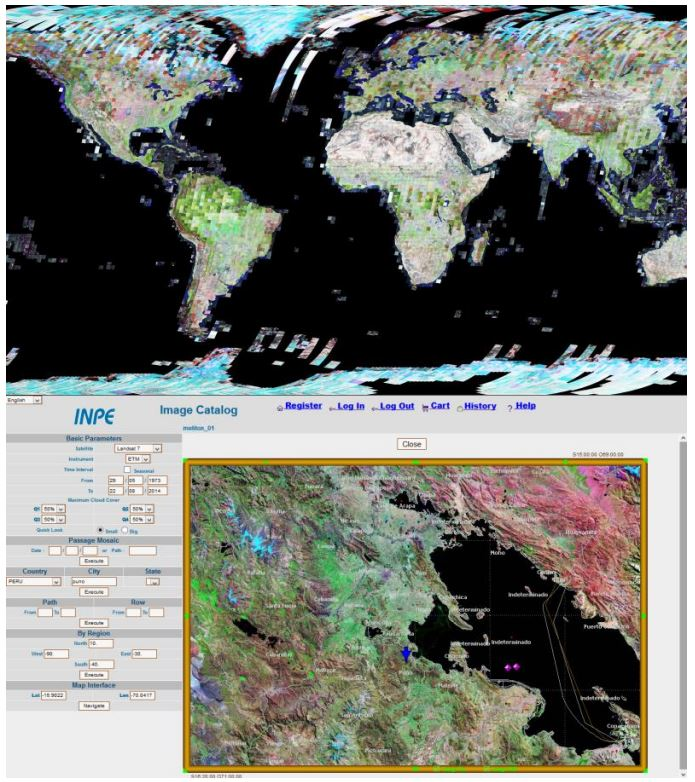
\includegraphics[width=7cm, height=8cm]{figuras/1.JPG}
            \caption{Catalogo de imágenes INPE}
            \label{f1} 
            \end{center}
    \end{figure}
    \item {\textbf{Método de tratamiento de datos}}\par
    El tratamiento de las imágenes satelitales comprende dos pasos, el primero trata las imágenes mediante el software AGKM implementado en lenguaje Matlab. Este software tiene implementado los algoritmos K-medias y AGKM, a partir del procesamiento con este software es que se obtiene la entropía de cada imagen las que fueron almacenadas en una tabla y posteriormente evaluadas estadísticamente con asistencia del SPSS para probar la eficacia del algoritmo. \par
    El algoritmo propuesto es el AGKM compuesto de dos partes, la primera parte se encarga de buscar el número ideal de conglomerados en la imagen satelital(Ver Figura ~\ref{f2}.) por medio de los Algoritmos Genéticos (valor de inicialización para Kmedias), la segunda parte comprende el algoritmo K-medias que utiliza como entrada el número de conglomerados encontrados por los algoritmos genéticos.
    \begin{figure}[H]
        \begin{center}
            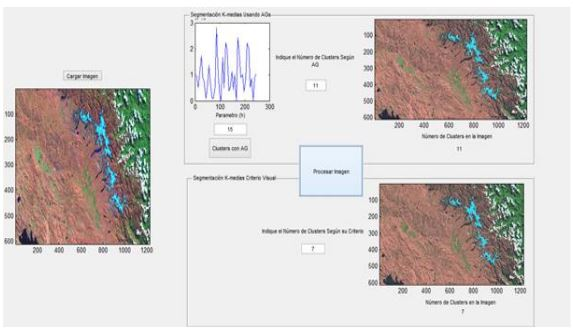
\includegraphics[width=8cm, height=5.5cm]{figuras/2.JPG}
            \caption{Máscara de la aplicación AGKM}
            \label{f2} 
            \end{center}
    \end{figure}
\end{itemize}
Finalmente, en la tesis anteiormente mencionada se implementó un aplicación usando la metodología de los Algoritmos Genéticos (AGs) y K-medias, el primero tiene la finalidad de encontrar un número de conglomerados existentes en la imagen y el segundo realiza el proceso de separación. La métrica usada para evaluar la eficiencia de este algoritmo es el valor de la entropía en las imágenes, los resultados obtenidos son sometidos a una prueba estadística que nos indica que existe una ligera mejoría.
Y se concluyó que el AGKM ofrece una ligera mejoría con respecto al algoritmo K-medias tradicional en la segmentación de imágenes satelitales para la Región Puno.\par

\item En la tesis titulada \textit{\textbf{“Aplicación de Algoritmos Inteligentes para Reconocimiento Automático de Enfermedades Foliares de Cultivo de Palta”}} \citep{castro} se aplicaron cuatro algoritmos inteligentes: Naive Bayes, Random forest, Redes Neuronales y Support Vector Machines y tuvo como objetivo general la determinación del algoritmo inteligente más eficaz para el reconocimiento de imágenes de la enfermedad foliar de palta.
\begin{itemize}
    \item {\textbf{Técnica para recopilación de datos}}\par
    Se realizó un muestreo sistemático de grilla sobre la ubicación geográfica de los cultivos de palta hasta recolectar un total de 630 muestras enfermas y sanas.
    \item {\textbf{Instrumento para recopilación de datos}}\par
    Cámara fotográfica profesional - CANÓN EOS REBEL T5I (Full HD + HDMI) – Para recolección de datos.(Ver Figura ~\ref{f3} y ~\ref{f4}.).
    \item {\textbf{Adquisición de datos}}\par
    Se hizo el uso de Cámara fotográfica profesional - CANÓN EOS REBEL T5I (Full HD + HDMI) para adquisición de imágenes sanas y enfermas (Oligonychus sp.).
    \begin{figure}[H]
        \begin{center}
            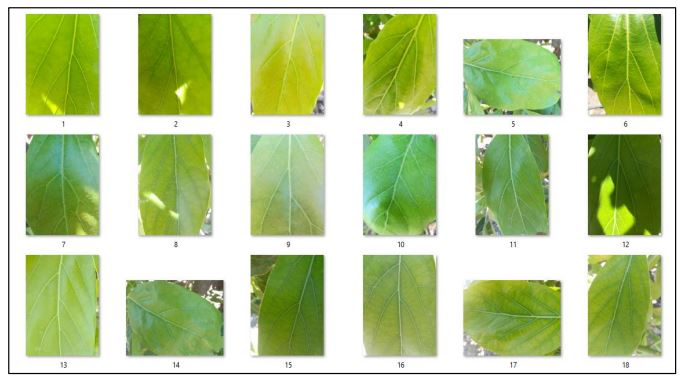
\includegraphics[width=8cm, height=5cm]{figuras/3.JPG}
            \caption{Se recolecto en total 330 imágenes sanas (se adjunta algunas imágenes)}
            \label{f3} 
            \end{center}
    \end{figure}
        \begin{figure}[H]
        \begin{center}
            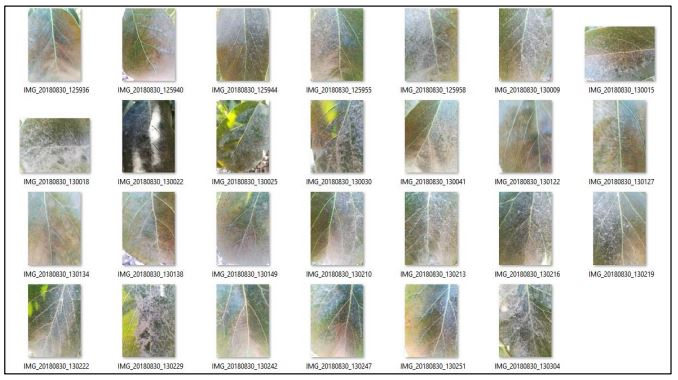
\includegraphics[width=8cm, height=5cm]{figuras/4.JPG}
            \caption{Se recolecto en total 300 imágenes enfermas (Oligonychus sp.), se adjunta algunas imágenes}
            \label{f4} 
            \end{center}
    \end{figure}
    \item {\textbf{Reconocimiento de datos}}\par
    En esta fase se realizó el entrenamiento de los modelos y la evaluación de la exactitud. (Ver Figura ~\ref{f5}) Se utilizaron 4 algoritmos: Redes Neuronales, Support Vector Machines y Random Forest, Naive Bayes. La matriz con los valores extraídos de las subimágenes se particionó en dos partes de manera aleatoria: 80\% de las observaciones (filas de la matriz) para entrenamiento de los modelos (dataset de entrenamiento), y 20\% de las observaciones para validación de los modelos (dataset de validación). El dataset de entrenamiento se usó entonces para entrenar los 4 modelos. Una vez que se entrenó el modelo para cada clasificador, se usó el dataset de validación para evaluar la exactitud del modelo respectivo, comparando la clase de referencia de cada observación (‘enferma’ o ‘sana’) con la clase predicha por el clasificador.
    \begin{figure}[H]
        \begin{center}
            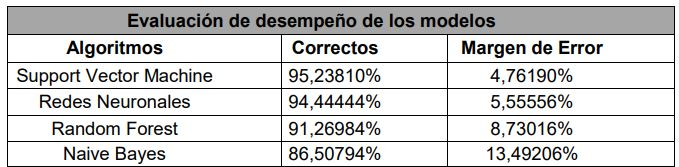
\includegraphics[width=8cm, height=3cm]{figuras/5.JPG}
            \caption{Evaluación de desempeño de modelos}
            \label{f5} 
            \end{center}
    \end{figure}
    
\end{itemize}

Luego de la evaluación de su eficacia se obtuvo que el algoritmo Maquina de Soporte Vectorial tiene mayor asertividad de 96\% en el reconocimiento de enfermedades foliares del cultivo de palta, esto después de ser evaluados con Matriz de Confusión.
\end{enumerate}
\section{\textbf{Conclusiones}}
Este informe presentó información relevante respecto a dos ejemplos de instrumentos de recolección de datos en informática o en ciencias de la computación. Se ha explicado para cada una de las investigaciones en que consistió su trabajo, el instrumento, método o técnica que usaron y finalmente que se logró con ello, además de permitir reafirmar que la informática es un campo futurista avanzado y emergente de innovaciones importantes relacionadas con la forma de vida moderna. 
%-------------------------------------------------------
\medskip
\bibliography{refer}
\end{document}
